\documentclass[11pt,a4paper]{article}

% ---------- Sprache & Encoding ----------
\usepackage[utf8]{inputenc}
\usepackage[T1]{fontenc}
\usepackage{lmodern}

% ---------- Layout ----------
\usepackage[a4paper,margin=2.3cm]{geometry}
\usepackage{enumitem}
\usepackage{booktabs}
\usepackage{array}
\usepackage{tabularx}
\usepackage{graphicx}
\usepackage{amsmath,amssymb}
\usepackage{xcolor}
\usepackage{tcolorbox}
\tcbuselibrary{skins,breakable}
\usepackage{fancyhdr}
\usepackage[hidelinks]{hyperref}
\usepackage{titlesec}
\usepackage{tikz}

% ---------- Farben ----------
\definecolor{kfrblue}{HTML}{1F5C99}
\definecolor{warnorange}{HTML}{B45309}
\definecolor{warnbg}{HTML}{FFF3E0}
\definecolor{tipbg}{HTML}{EAF3EA}
\definecolor{tipgreen}{HTML}{2E7D32}

% ---------- Überschriften ----------
\titleformat{\section}{\large\bfseries\color{kfrblue}}{\thesection}{0.6em}{}
\titleformat{\subsection}{\normalsize\bfseries\color{kfrblue}}{\thesubsection}{0.6em}{}

% ---------- Kopf-/Fusszeile ----------
\pagestyle{fancy}
\fancyhf{}
\renewcommand{\headrulewidth}{0.4pt}
\fancyhead[L]{\small Physik 5.\,Klasse, Praktikum 01}
\fancyhead[R]{\small Spezifische W\"armekapazit\"at eines Metalls}
\fancyfoot[C]{\small\thepage}

% ---------- Boxen ----------
\newtcolorbox{achtungbox}[1][]{%
  colback=warnbg, colframe=warnorange, coltitle=white, colbacktitle=warnorange,
  boxrule=0.8pt, arc=2pt,
  left=6pt, right=6pt, top=4pt, bottom=4pt, breakable,
  title={\textbf{Achtung: darauf kommt es an}#1},
  fonttitle=\small, fontupper=\small
}
\newtcolorbox{tippbox}[1][]{%
  colback=tipbg, colframe=tipgreen, coltitle=white, colbacktitle=tipgreen,
  boxrule=0.8pt, arc=2pt,
  left=6pt, right=6pt, top=4pt, bottom=4pt, breakable,
  title={\textbf{Merke}#1},
  fonttitle=\small, fontupper=\small
}
\newtcolorbox{aufgabebox}[1][]{%
  colback=gray!6, colframe=kfrblue, coltitle=white, colbacktitle=kfrblue,
  boxrule=0.8pt, arc=2pt,
  left=6pt, right=6pt, top=4pt, bottom=4pt, breakable,
  title={\textbf{Aufgabe}#1},
  fonttitle=\small, fontupper=\small
}

\setlist[itemize]{leftmargin=1.4em, itemsep=2pt, topsep=3pt}
\setlist[enumerate]{leftmargin=1.6em, itemsep=2pt, topsep=3pt}

\newcommand{\Temp}{T}

% ---------- einfache Einheiten-Makros (kein siunitx nötig) ----------
\newcommand{\celsius}{\ensuremath{^{\circ}\mathrm{C}}}
\newcommand{\kelvin}{K}
\newcommand{\kilogram}{kg}
\newcommand{\SI}[2]{#1\,#2}

% ---------- Platz für handschriftliche Antworten (kariert, für Rechnungen geeignet) ----------
\newlength{\gridwidth}
\newcommand{\antwortraum}[1]{%
  \par\vspace{4pt}\noindent
  \setlength{\gridwidth}{\linewidth}%
  \begin{tikzpicture}
    \draw[step=0.5cm, gray!25, very thin] (0,0) grid (\gridwidth,#1);
    \draw[black, thin] (0,0) rectangle (\gridwidth,#1);
  \end{tikzpicture}
  \vspace{4pt}
}
\newcommand{\antwortraumS}{\antwortraum{2.5cm}}
\newcommand{\antwortraumM}{\antwortraum{4.5cm}}
\newcommand{\antwortraumL}{\antwortraum{8cm}}

% ---------- Platz für Zeichnungen ----------
\newcommand{\zeichenraum}[1][4.5cm]{%
  \par\vspace{4pt}\noindent
  \fbox{\begin{minipage}[t][#1][t]{\dimexpr\linewidth-2\fboxsep-2\fboxrule}\ \end{minipage}}
  \vspace{4pt}
}

\begin{document}
\thispagestyle{empty}

% ---------- Titelblock ----------
\begin{center}
  {\color{kfrblue}\Large\bfseries Praktikum 01: Spezifische W\"armekapazit\"at eines Metalls}\\[2pt]
  {\normalsize Kantonsschule Freudenberg, Physik 5.\ Klasse}
\end{center}

\vspace{4pt}
\noindent
\begin{tabularx}{\linewidth}{@{}X X@{}}
  Name/n: \dotfill & Datum: \dotfill \\[4pt]
  Halbklasse: \dotfill & Unterlagen von: L.\,Keller \\
\end{tabularx}

\vspace{10pt}
\hrule
\vspace{10pt}

% ======================================================
\section{Ziel}
Ziel dieses Versuchs ist die Messung der spezifischen W\"armekapazit\"at einer unbekannten Metallprobe. Dazu wird die Probe auf eine Temperatur von knapp \SI{100}{\celsius} gebracht und anschliessend in einem Kalorimeter (isoliertes Kupfergef\"ass) mit Wasser abgek\"uhlt.

Die gespeicherte thermische Energie, welche die Metallprobe mit sich bringt, ist verkn\"upft mit der spezifischen W\"armekapazit\"at des Metalls. Deshalb kann \"uber eine Energiebetrachtung und mittels Messung der Endtemperatur des Wassers die spezifische W\"armekapazit\"at des Metalls bestimmt werden. Die erforderliche Gleichung leitest du am Schluss in der Auswertung selbst her, wenn du alle Messgr\"ossen kennst.

F\"ur diese Berechnung werden die spezifischen W\"armekapazit\"aten von Wasser und Kupfer aus einer Tabelle entnommen. Aufgrund der ermittelten spezifischen W\"armekapazit\"at soll das unbekannte Metall der Probe bestimmt werden; zus\"atzlich soll die Hypothese mit Hilfe einer Dichtebestimmung validiert werden. Schliesslich wird die Abweichung vom Literaturwert mit einer Fehlerrechnung diskutiert.

% ======================================================
\section{Theorie}
\label{sec:theorie}
Dieses Kapitel enth\"alt alle Grundlagen, die du f\"ur den Versuch brauchst. Je nachdem, in welcher Klasse ihr dieses Praktikum durchf\"uhrt, wurde das Thema W\"arme und Thermodynamik im Unterricht bereits behandelt oder noch nicht. Lies dieses Kapitel deshalb in jedem Fall sorgf\"altig durch, egal ob als Wiederholung oder als Einf\"uhrung, bevor du mit dem Versuch startest.

\subsection{Temperatur und W\"arme}
Alle Stoffe bestehen aus Teilchen (Atome, Molek\"ule), die sich st\"andig bewegen. Die \emph{Temperatur} $\Temp$ eines K\"orpers ist ein Mass f\"ur die mittlere Bewegungsenergie dieser Teilchen: Je schneller sich die Teilchen im Mittel bewegen, desto h\"oher ist die Temperatur.

Bringt man zwei K\"orper unterschiedlicher Temperatur in Kontakt, so \"ubertragen die schnelleren Teilchen des w\"armeren K\"orpers Bewegungsenergie an die langsameren Teilchen des k\"alteren K\"orpers. Diese \"ubertragene Energie nennt man \emph{W\"arme} $Q$. Wichtig ist der Unterschied zwischen den beiden Begriffen:
\begin{itemize}
  \item Die \textbf{Temperatur} $\Temp$ beschreibt einen \emph{Zustand} (wie warm ein K\"orper gerade ist).
  \item Die \textbf{W\"arme} $Q$ beschreibt eine \emph{Energiemenge}, die von einem K\"orper zum anderen \"ubertragen wird.
\end{itemize}

\subsection{Spezifische W\"armekapazit\"at}
F\"uhrt man einem K\"orper eine W\"armemenge $Q$ zu, so erh\"oht sich seine Temperatur um $\Delta\Temp$. (Vorausgesetzt, es findet dabei kein Phasen\"ubergang statt, z.\,B.\ Schmelzen.) Wie stark die Temperatur ansteigt, h\"angt von zwei Dingen ab: von der Masse $m$ des K\"orpers und von seiner \emph{spezifischen W\"armekapazit\"at} $c$, einer Materialkonstante. Es gilt:
\[
  Q = m \cdot c \cdot \Delta\Temp, \qquad [c] = \mathrm{J\,kg^{-1}\,K^{-1}}
\]
Die spezifische W\"armekapazit\"at gibt an, wie viel Energie n\"otig ist, um \SI{1}{\kilogram} eines Stoffes um \SI{1}{\kelvin} zu erw\"armen. Ein Stoff mit grossem $c$ kann viel W\"arme speichern, ohne dass seine Temperatur stark steigt; ein Stoff mit kleinem $c$ erw\"armt sich (und k\"uhlt sich ab) viel schneller.

\begin{center}
\renewcommand{\arraystretch}{1.25}
\begin{tabularx}{0.9\linewidth}{@{}Xll@{}}
  \toprule
  \textbf{Stoff} & \textbf{spez.\ W\"armekapazit\"at $c$ in $\mathrm{J\,kg^{-1}\,K^{-1}}$} & \textbf{Dichte $\rho$ in $\mathrm{g/cm^3}$} \\
  \midrule
  Wasser & $4190$ & $1.00$ \\
  Aluminium & $897$ & $2.70$ \\
  Nickel & $444$ & $8.91$ \\
  Kupfer & $385$ & $8.96$ \\
  Messing & $\approx 380$ & $\approx 8.50$ \\
  Zink & $388$ & $7.14$ \\
  \bottomrule
\end{tabularx}
\end{center}
\emph{Hinweis:} Diese Tabelle hilft dir sp\"ater beim Bestimmen des unbekannten Metalls. Wasser hat eine ungew\"ohnlich grosse spezifische W\"armekapazit\"at; Metalle liegen alle deutlich tiefer. Nickel und Kupfer haben eine \"ahnliche Dichte, Kupfer und Messing eine \"ahnliche spezifische W\"armekapazit\"at: erst die Kombination beider Messgr\"ossen identifiziert das Metall eindeutig. Zink kommt in diesem Praktikum nicht als Probe vor, ist aber zum Vergleich mit aufgef\"uhrt.

\textbf{Kleines Rechenbeispiel:} Wie viel W\"arme braucht es, um $0.5\ \mathrm{kg}$ Wasser um $20\ \mathrm{K}$ zu erw\"armen?
\[
  Q = m \cdot c \cdot \Delta\Temp = 0.5\ \mathrm{kg} \cdot 4190\ \mathrm{J\,kg^{-1}\,K^{-1}} \cdot 20\ \mathrm{K} = 41\,900\ \mathrm{J}.
\]

\begin{aufgabebox}
Wasser hat mit $\mathrm{4190\ J\,kg^{-1}\,K^{-1}}$ eine der h\"ochsten spezifischen W\"armekapazit\"aten aller bekannten Stoffe, deutlich h\"oher als die der Metalle in der Tabelle oben. \"Uberlegt euch: Weshalb ist genau diese Eigenschaft von Wasser (in Ozeanen, Seen, aber auch im K\"orper) wichtig f\"ur unser Klima? Was w\"are anders, h\"atte Wasser eine \"ahnlich kleine spezifische W\"armekapazit\"at wie ein Metall?
\end{aufgabebox}
\antwortraumM

\subsection{Energieerhaltung beim Mischungskalorimeter}
Bringt man zwei K\"orper unterschiedlicher Temperatur in Kontakt, tauschen sie so lange W\"arme aus, bis sich eine gemeinsame \emph{Mischtemperatur} einstellt. Findet dieser Ausgleich (n\"aherungsweise) ohne W\"armeverluste an die Umgebung statt, gilt der Energieerhaltungssatz in der Form
\[
  Q_{\text{abgegeben}} = Q_{\text{aufgenommen}}.
\]
Ein einfaches Beispiel zur Veranschaulichung: Mischt man warmes Wasser mit kaltem Wasser, so gibt das warme Wasser genau so viel W\"arme ab, wie das kalte Wasser aufnimmt, bis beide die gleiche Mischtemperatur haben.

\paragraph{Das System: drei K\"orper, zwei Zeitpunkte.}
In unserem Versuch tauschen \emph{drei} K\"orper W\"arme miteinander aus:
\begin{itemize}
  \item die Metallprobe (Masse $m_M$, spezifische W\"armekapazit\"at $c_M$: die gesuchte Gr\"osse),
  \item das Wasser \emph{im Kalorimeter} (Masse $m_W$, spezifische W\"armekapazit\"at $c_W$ aus der Tabelle),
  \item das Kalorimetergef\"ass selbst (Masse $m_K$, spezifische W\"armekapazit\"at $c_K$ von Kupfer aus der Tabelle).
\end{itemize}
Die Energiebilanz betrachtet genau dieses System aus drei K\"orpern, unter der (idealisierenden) Annahme, dass w\"ahrend des Mischvorgangs keine W\"arme an die Umgebung entweicht, das Kalorimeter also perfekt isoliert w\"are. Wie gut diese Annahme tats\"achlich zutrifft, wird sp\"ater bei den Fehlerquellen diskutiert (Abschnitt~\ref{sec:fehlerquellen}).

Massgebend f\"ur die Bilanz sind jeweils zwei Zeitpunkte:
\begin{itemize}
  \item \textbf{Vor dem Einf\"ullen}: Die Metallprobe hat ihre hohe Ausgangstemperatur $\Temp_{M0}$. Wasser und Kalorimetergef\"ass sitzen schon die ganze Zeit zusammen im Kalorimeter und haben deshalb beide dieselbe, tiefere Temperatur $\Temp_{W0}=\Temp_{K0}$.
  \item \textbf{Bei der Mischtemperatur}: Sobald sich Wasser, Gef\"ass und Metallprobe ausgeglichen haben, haben alle drei dieselbe Temperatur $\Temp_{M1}=\Temp_{W1}=\Temp_{K1}$.
\end{itemize}

\begin{achtungbox}[: Welches Wasser ist gemeint?]
Mit der Masse $m_W$ ist ausschliesslich das kleine bisschen destillierte Wasser \emph{im Kalorimeter} gemeint (ca.\ 1--1.5\,dl, das ihr selbst einf\"ullt und w\"agt), \textbf{nicht} das grosse gemeinsame Wasserbad, in dem die Kupfert\"opfe aufgeheizt werden. Das Wasserbad dient nur dazu, die Metallprobe indirekt zu erw\"armen (Abschnitt~\ref{sec:erwaermung}); mit dem Kalorimeter kommt es nie in Kontakt und taucht deshalb in dieser Energiebilanz gar nicht auf.
\end{achtungbox}

\begin{center}
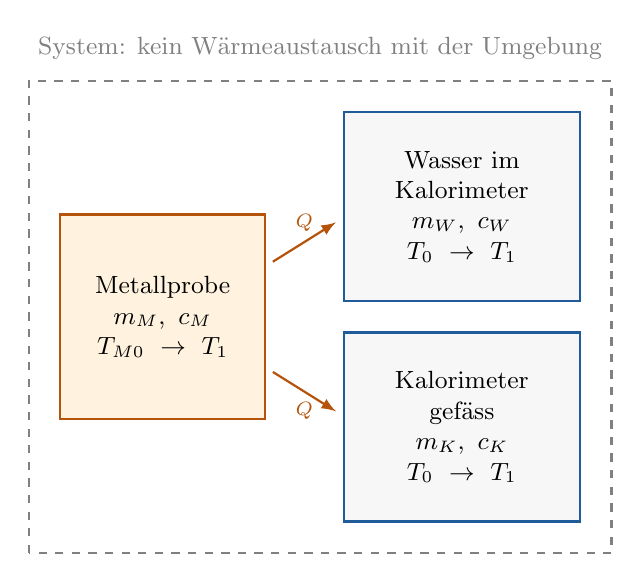
\begin{tikzpicture}[scale=1,every node/.style={font=\small,align=center}]
  \draw[dashed, thick, gray] (-0.4,0.0) rectangle (7.0,6.0);
  \node[gray, anchor=south] at (3.3,6.15) {System: kein W\"armeaustausch mit der Umgebung};

  \draw[thick, warnorange, fill=warnbg] (0,1.7) rectangle (2.6,4.3);
  \node at (1.3,3.0) {Metallprobe\\$m_M,\ c_M$\\$\Temp_{M0}\ \rightarrow\ \Temp_{1}$};

  \draw[thick, kfrblue, fill=gray!6] (3.6,3.2) rectangle (6.6,5.6);
  \node at (5.1,4.4) {Wasser im\\Kalorimeter\\$m_W,\ c_W$\\$\Temp_{0}\ \rightarrow\ \Temp_{1}$};

  \draw[thick, kfrblue, fill=gray!6] (3.6,0.4) rectangle (6.6,2.8);
  \node at (5.1,1.6) {Kalorimeter\-\\gef\"ass\\$m_K,\ c_K$\\$\Temp_{0}\ \rightarrow\ \Temp_{1}$};

  \draw[-latex, thick, warnorange] (2.7,3.7) -- node[above, warnorange, font=\scriptsize] {$Q$} (3.5,4.2);
  \draw[-latex, thick, warnorange] (2.7,2.3) -- node[below, warnorange, font=\scriptsize] {$Q$} (3.5,1.8);
\end{tikzpicture}
\end{center}
\noindent Dabei steht $\Temp_{0}:=\Temp_{W0}=\Temp_{K0}$ f\"ur die gemeinsame Anfangstemperatur von Wasser und Gef\"ass, und $\Temp_{1}:=\Temp_{M1}=\Temp_{W1}=\Temp_{K1}$ f\"ur die gemeinsame Mischtemperatur am Ende.

\paragraph{Woher die beiden Seiten der Gleichung kommen.}
Jeder der drei K\"orper liefert nach der Definition aus Abschnitt~2.2 einen Term der Form $Q=mc\,\Delta\Temp$. Die Metallprobe ist der einzige K\"orper, der abk\"uhlt und Energie abgibt; sie steht deshalb allein auf der linken Seite. Wasser und Kalorimetergef\"ass erw\"armen sich beide und nehmen Energie auf; sie stehen deshalb gemeinsam (addiert) auf der rechten Seite:
\[
  \underbrace{m_M\,c_M\,(\Temp_{M0}-\Temp_1)}_{Q_{\text{abgegeben, Metallprobe}}} \ =\ \underbrace{m_W\,c_W\,(\Temp_1-\Temp_{W0}) + m_K\,c_K\,(\Temp_1-\Temp_{K0})}_{Q_{\text{aufgenommen, Wasser und Gef\"ass}}}.
\]
Bei der Reihenfolge innerhalb jeder Klammer gilt dieselbe Regel wie beim Zweik\"orper-Beispiel weiter oben: Man schreibt jeweils die \emph{h\"ohere} Temperatur zuerst, damit $\Delta\Temp$ positiv wird und die Klammer tats\"achlich die abgegebene bzw.\ aufgenommene W\"armemenge darstellt (keine negative Zahl). Bei der Metallprobe ist das die Anfangstemperatur $\Temp_{M0}$ (sie ist die heisseste), bei Wasser und Gef\"ass ist es die Endtemperatur $\Temp_1$ (sie erw\"armen sich ja erst auf diesen Wert).

Diese Gleichung ist der Ausgangspunkt f\"ur die Auswertung: Um daraus eine Formel f\"ur die gesuchte Gr\"osse $c_M$ zu erhalten, musst du sie noch nach $c_M$ aufl\"osen, sobald du alle Messgr\"ossen kennst (siehe Auswertung).

\subsection{Warum indirekte Erw\"armung?}
Die Metallprobe wird nicht direkt im Wasserbad, sondern in einem separaten Kupfertopf erw\"armt (siehe Abschnitt~\ref{sec:erwaermung}). \"Uberlege dir beim Versuch, welche Vorteile das gegen\"uber einer direkten Erw\"armung im Wasser hat. Die Antwort ist Teil der Auswertung.

% ======================================================
\section{Sicherheitshinweise}
\begin{itemize}
  \item Das Wasserbad und die Kupfert\"opfe werden bis nahe \SI{100}{\celsius} erhitzt. \textbf{Nicht} mit blossen H\"anden anfassen, sondern Topflappen/Zange verwenden.
  \item Die Metallprobe nach der Entnahme aus dem Wasserbad ist ebenfalls hei\ss{}: zügig, aber kontrolliert transportieren.
  \item Kochplatte nach Gebrauch ausschalten; Vorsicht vor Spritzwasser auf der heissen Platte.
\end{itemize}

% ======================================================
\section{Material}

\paragraph{Lehrperson (1$\times$):}
\begin{itemize}
  \item Kochplatte, grosser Topf mit Deckel und Kupferpfannen, Thermometer (bis \SI{110}{\celsius})
  \item Metallproben (als kleine Pellets/Granulat, kein durchgehender Block): Aluminium, Nickel, Kupfer, Messing
  \item Haartrockner
  \item 1 \"Uberlaufgef\"ass
\end{itemize}

\paragraph{Sch\"ulerinnen und Sch\"uler (6 Stationen):}
\begin{itemize}
  \item Kalorimeter (mit R\"uhrwerkzeug) und Holzklotz als Unterlage
  \item Zwei Bechergl\"aser (\SI{400}{ml})
  \item Thermometer (bis \SI{100}{\celsius})
  \item Lupe
\end{itemize}

% ======================================================
\section{Durchf\"uhrung}

\subsection{Erw\"armung der Metallprobe}
\label{sec:erwaermung}
Die Erw\"armung wird von der Lehrperson f\"ur alle Gruppen gemeinsam durchgef\"uhrt: Alle Kupfert\"opfe stehen zusammen in einem grossen, mit Wasser gef\"ullten Topf auf einer einzigen Kochplatte und werden gleichzeitig erhitzt. Eure Aufgabe als Gruppe beschr\"ankt sich auf die Vorbereitung und das Ablesen.

\begin{center}
  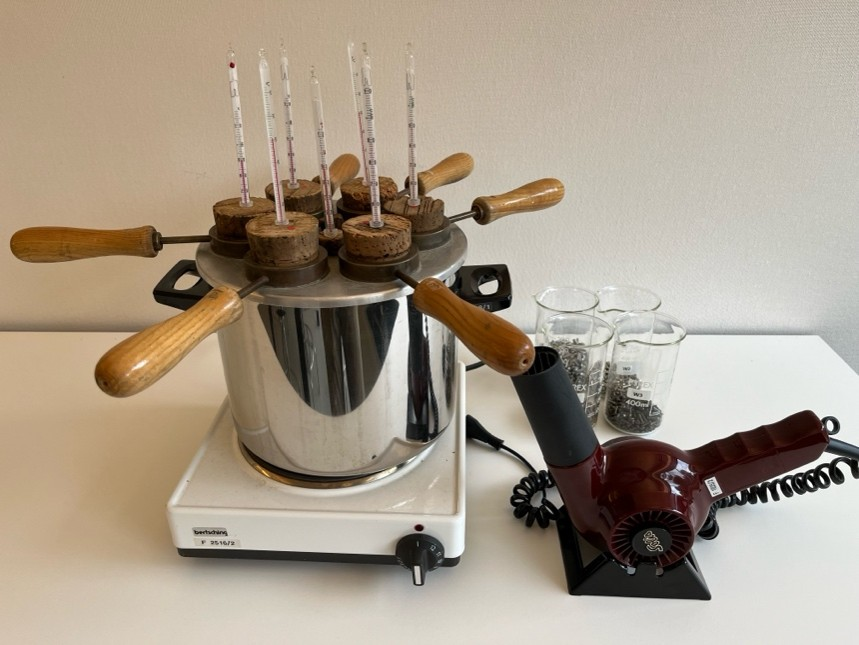
\includegraphics[width=0.62\linewidth]{Wassertopf.jpg}\\
  {\small\itshape Gemeinsames Wasserbad mit den Kupfert\"opfen (Thermometer stecken in Korkstopfen), daneben Metallproben als Pellets in Bechergl\"asern und Haartrockner.}
\end{center}

\begin{enumerate}
  \item F\"ulle von den Pellets des gew\"ahlten Metalls eine Menge ein, die ca.\ \SI{1}{cm} des Bodens des Kalorimeters bedeckt.
  \item W\"age die Metallprobe, \emph{bevor} sie in euren Kupfertopf eingef\"ullt wird, und trage den Messwert $m_M$ ins Messprotokoll ein.
  \item Gebt euren Kupfertopf mit der Metallprobe der Lehrperson ab. Sie stellt alle Kupfert\"opfe zusammen ins Wasserbad und heizt es auf der Kochplatte auf.
  \item Sobald die Kupfert\"opfe im Wasserbad stehen, lest ihr laufend zwei Temperaturen ab: die Temperatur im \emph{Inneren eures eigenen Kupfertopfs} $\Temp_{KT}$ und die Temperatur des gemeinsamen Wasserbads $\Temp_{WB}$ (an der Lehrpersonen-Station angeschrieben bzw.\ vorgelesen).
\end{enumerate}

\begin{achtungbox}
\begin{itemize}
  \item \textbf{Die richtige Temperatur ablesen:} Massgebend f\"ur eure Metallprobe ist die Temperatur \emph{im Kupfertopf} $\Temp_{KT}$, nicht die Temperatur des Wassers im grossen Topf $\Temp_{WB}$. Das Wasser im grossen Topf ist nur das Heizbad; eure Probe befindet sich im Kupfertopf und nimmt dessen Temperatur an.
  \item \textbf{Geduld:} Nehmt die Probe \textbf{nicht zu fr\"uh} heraus. Eure Probe liegt als lose Sch\"uttung aus Pellets im Kupfertopf, nicht als ein einzelner Block: die Pellets ber\"uhren sich nur an einzelnen Punkten, dazwischen liegt Luft, die W\"arme viel schlechter leitet als Metall. Deshalb breitet sich die W\"arme in der Sch\"uttung langsamer aus als in einem massiven St\"uck, Pellets nahe der Topfwand k\"onnen schon w\"armer sein als Pellets in der Mitte. Wartet, bis sich $\Temp_{WB}$ und $\Temp_{KT}$ nicht mehr merklich einander ann\"ahern, das dauert erfahrungsgem\"ass mindestens 8--10 Minuten. Auch dann bleibt meist noch eine kleine Restdifferenz zwischen den beiden Anzeigen bestehen, mehr Wartezeit bringt dann nichts mehr.
\end{itemize}
\end{achtungbox}

\begin{enumerate}[resume]
  \item Sobald sich die Temperaturen nicht mehr merklich \"andern, gilt als Ausgangstemperatur der Metallprobe
  \[
    \Temp_{M0} = \frac{\Temp_{WB} + \Temp_{KT}}{2}.
  \]
  \item Mach eine Querschnittszeichnung von Wasserbad, Kupfertopf und Metallprobe (als Pellet-Sch\"uttung) sowie den beiden Thermometern.
\end{enumerate}
\zeichenraum

\begin{aufgabebox}
Wieso reicht es nicht, die Temperatur der Probe (bzw.\ $\Temp_{KT}$) irgendwann w\"ahrend des Aufheizens einmal zu messen und die Probe dann einfach z\"ugig ins Kalorimeter zu geben, statt zu warten, bis sich $\Temp_{WB}$ und $\Temp_{KT}$ nicht mehr merklich ann\"ahern? Was k\"onnte an einer solchen fr\"uhen Einzelmessung problematisch sein?
\end{aufgabebox}
\antwortraumM

\begin{aufgabebox}
Auch nach ausreichender Wartezeit bleibt zwischen $\Temp_{WB}$ und $\Temp_{KT}$ meist eine kleine Restdifferenz bestehen. Lest eure eigene Restdifferenz an euren beiden Thermometern ab (sie h\"angt u.\,a.\ davon ab, wie fein die Pellets verteilt sind) und \"uberlegt euch: Welchen Einfluss hat diese Restdifferenz auf euer Resultat f\"ur $c_M$? Wo taucht sie in eurer Fehlerrechnung auf, und wie sch\"atzt ihr daraus die Messgenauigkeit von $\Temp_{M0}$ ab?
\end{aufgabebox}
\antwortraumM

\begin{aufgabebox}
Warum wird die Metallprobe indirekt in einem Kupfertopf erw\"armt (statt in direktem Kontakt mit dem Wasser des Wasserbads)? Notiere mindestens zwei Gr\"unde.
\end{aufgabebox}
\antwortraumM

\subsection{Abk\"uhlung der Metallprobe im Kalorimeter}
Das Kalorimeter ist ein Kupfergef\"ass mit einer Doppelwandisolation, damit m\"oglichst wenig W\"arme vom Inneren des Gef\"asses an die Umgebung verloren geht.

\begin{center}
  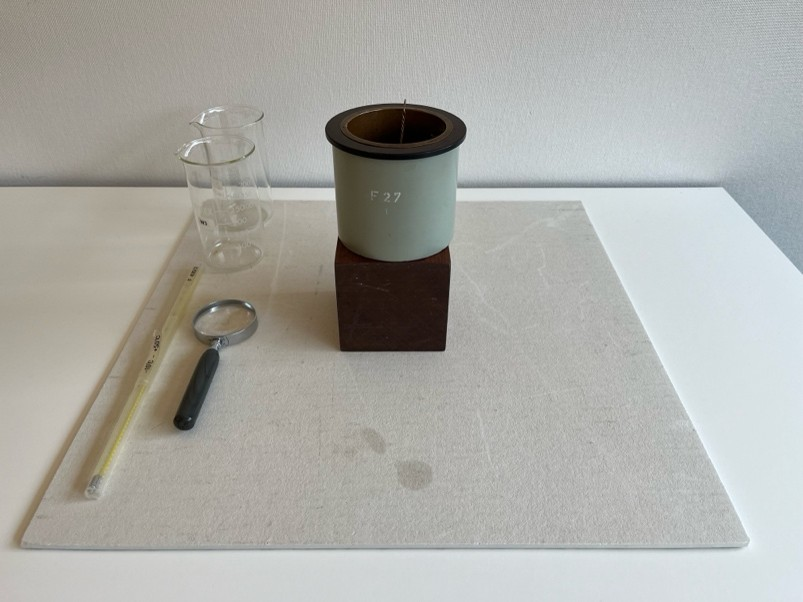
\includegraphics[width=0.55\linewidth]{Kalorimeter.jpg}\\
  {\small\itshape Eure Station: Kalorimeter auf Holzklotz, zwei Bechergl\"aser, Thermometer und Lupe.}
\end{center}

\begin{enumerate}
  \item Mach eine vereinfachte Querschnittszeichnung des Kalorimeters, inkl.\ Thermometer.
  \item W\"age den Kupferteil des Kalorimeters, der mit dem Wasser in Kontakt sein wird (inkl.\ R\"uhrwerkzeug), und trage die Masse $m_K$ ins Messprotokoll ein.
  \item F\"uge ca.\ 1--1.5\,dl \textbf{destilliertes} Wasser in das Kalorimeter und w\"age das Wasser (Masse $m_W$).
  \item Setze das Thermometer ein und lies die Anfangstemperatur des Wassers bzw.\ des Kalorimeters ab ($\Temp_{W0} = \Temp_{K0}$).
\end{enumerate}
\zeichenraum

\begin{aufgabebox}
F\"ur das Kalorimeter wird destilliertes statt gew\"ohnliches Leitungswasser verwendet. Wieso ist das f\"ur diesen Versuch wichtig?
\end{aufgabebox}
\antwortraumS

\begin{enumerate}[resume]
  \item Nehmt euren Kupfertopf mit Topflappen oder Zange aus dem gemeinsamen Wasserbad und gebt die Metallprobe zügig und vollständig in euer vorbereitetes Kalorimeter (siehe Achtungbox unten für Details).
  \item R\"uhrt das Wasser leicht um und beobachtet die Temperatur, bis sie ihr Maximum erreicht. Notiert diese Mischungstemperatur $\Temp_{W1} = \Temp_{K1} = \Temp_{M1}$ ins Messprotokoll.
\end{enumerate}

\begin{achtungbox}
\begin{itemize}
  \item \textbf{Z\"ugig transportieren:} F\"uge die Metallprobe schnell dem Wasser zu, sodass kein Wasser wegspritzt und die Metallprobe m\"oglichst wenig W\"arme an die Umgebungsluft verliert. Jede Sekunde an der Luft k\"uhlt die Probe unkontrolliert ab, bevor sie im Kalorimeter erfasst wird.
  \item \textbf{Vollst\"andig umf\"ullen:} Achte darauf, dass die \emph{ganze} gewogene Metallmenge im Kupfertopf tats\"achlich ins Kalorimeter gelangt. Bei den kleinen Pellets bleiben leicht einzelne St\"ucke am Topfrand oder -boden h\"angen, kontrolliere das sorgf\"altig. Zur\"uckbleibende R\"uckst\"ande verf\"alschen $m_M$.
  \item \textbf{R\"uhren:} Halte das Wasser mit dem R\"uhrwerkzeug stets in leichter Bewegung, damit im Wasser keine Temperaturunterschiede entstehen und das Thermometer nicht nur lokal misst.
  \item \textbf{Deckel/Isolation nutzen:} Halte das Kalorimeter w\"ahrend der Messung m\"oglichst geschlossen. Eine offene Wasseroberfl\"ache k\"uhlt zus\"atzlich durch Verdunstung ab.
  \item \textbf{Den richtigen Moment erwischen:} Beobachte, wie die Wassertemperatur $\Temp_W$ ansteigt. Sobald sie ihr Maximum erreicht hat (und schon fast wieder zu sinken beginnt), notiere die h\"ochste Temperatur, die sogenannte Mischungstemperatur $\Temp_{W1} = \Temp_{K1} = \Temp_{M1}$. Danach f\"allt die Temperatur wieder, weil das Kalorimeter selbst nie perfekt isoliert ist: Ein zu sp\"at abgelesener Wert liegt \textbf{systematisch zu tief}.
\end{itemize}
\end{achtungbox}

\begin{tippbox}
Wer unsicher ist, den exakten Umkehrpunkt zu treffen: Notiere die Temperatur alle 10--15\,s auch kurz \emph{vor} und \emph{nach} dem vermuteten Maximum. So l\"asst sich der h\"ochste Wert im Nachhinein sauber bestimmen, auch wenn der genaue Umkehrmoment beim Beobachten knapp verpasst wurde.
\end{tippbox}

% ======================================================
\section{Auswertung}
\label{sec:auswertung}
\begin{enumerate}
  \item Du kennst jetzt alle Messgr\"ossen. Leite eine Gleichung her, mit der sich die spezifische W\"armekapazit\"at $c_M$ der Metallprobe berechnen l\"asst (vgl.\ Abschnitt~2.3), und berechne damit $c_M$.
\end{enumerate}
\antwortraumL

\begin{enumerate}[resume]
  \item Du kennst bereits die Masse $m_M$ deiner Metallprobe. Um die Dichte zu bestimmen, fehlt dir noch das Volumen $V_M$. Deine Probe besteht aus vielen kleinen, unregelm\"assig geformten Pellets, ein Geodreieck oder eine Schieblehre helfen hier also nicht direkt weiter. \"Uberlege dir selbst eine Methode, wie du das Gesamtvolumen all deiner Pellets trotzdem messen kannst. An der Lehrpersonen-Station steht dir dazu Material zur Verf\"ugung, das du bei Bedarf anfordern kannst. Dokumentiere dein Vorgehen und berechne die Dichte.
\end{enumerate}
\antwortraumL

\begin{enumerate}[resume]
  \item Vergleiche deine spezifische W\"armekapazit\"at und Dichte mit Literaturwerten. Um welches Metall handelt es sich?
\end{enumerate}
\antwortraumM

\begin{aufgabebox}
Schaut euch die Skala eurer Thermometer genau an, bevor ihr die Messgenauigkeit im Messprotokoll festlegt. \"Uberlegt euch: Welche Genauigkeit ist f\"ur eure Temperaturmessungen realistisch, und wie wirkt sich diese Ablesegenauigkeit auf die berechnete spezifische W\"armekapazit\"at aus?
\end{aufgabebox}
\antwortraumS

\begin{enumerate}[resume]
  \item F\"uhre eine Fehlerrechnung durch, indem du die Messgenauigkeit deiner Messungen in der finalen Gleichung anschaust. Wie genau kann die berechnete Gr\"osse sein? Ist sie im Vergleich mit dem Literaturwert und unter Ber\"ucksichtigung des Fehlers gen\"ugend genau?
\end{enumerate}
\antwortraumL

\begin{enumerate}[resume]
  \item F\"uhre dieselbe Fehlerrechnung auch f\"ur deine Dichte $\rho_M=m_M/V_M$ durch. Wie genau ist dein Wert, und best\"atigt er dein Ergebnis aus Frage~3 auch unter Ber\"ucksichtigung des Fehlers?
\end{enumerate}
\antwortraumM

\begin{enumerate}[resume]
  \item Diskutiere deine Erkenntnisse sowie m\"ogliche Fehlerquellen (siehe auch Abschnitt~\ref{sec:fehlerquellen}).
\end{enumerate}
\antwortraumL

% ======================================================
\section{Messprotokoll}
\renewcommand{\arraystretch}{1.6}
\begin{center}
\begin{tabularx}{\linewidth}{@{}X p{6.1cm} p{2.6cm}@{}}
  \toprule
  \textbf{Gr\"osse} & \textbf{Messung} & \textbf{Messgenauigkeit} \\
  \midrule
  Masse der Metallprobe & $m_M =$\dotfill & $\pm$\dotfill \\
  Masse des Kalorimeters (Kupfer) & $m_K =$\dotfill & $\pm$\dotfill \\
  Masse des Wassers & $m_W =$\dotfill & $\pm$\dotfill \\
  Anfangstemperatur der Metallprobe & $\Temp_{M0} =$\dotfill & $\pm$\dotfill \\
  Anfangstemperatur Kalorimeter/Wasser & $\Temp_{K0} = \Temp_{W0} =$\dotfill & $\pm$\dotfill \\
  Mischungstemperatur (Endtemperatur) & $\Temp_{K1} = \Temp_{W1} = \Temp_{M1} =$\dotfill & $\pm$\dotfill \\
  Spez.\ W\"armekapazit\"at von Wasser & $c_W =$\dotfill & \\
  Spez.\ W\"armekapazit\"at von Kupfer & $c_K =$\dotfill & \\
  Volumen der Metallprobe & $V_M =$\dotfill & $\pm$\dotfill \\
  \bottomrule
\end{tabularx}
\end{center}

% ======================================================
\section{Fehlerquellen: worauf du achten solltest}
\label{sec:fehlerquellen}
Diese Liste fasst die wichtigsten Fehlerquellen dieses Versuchs zusammen und hilft dir bei der Diskussion in der Auswertung:

\begin{itemize}
  \item \textbf{W\"armeverlust beim Transfer:} Zwischen Herausnehmen der Probe aus dem Wasserbad und Eintauchen ins Kalorimeter geht immer etwas W\"arme an die Luft verloren. Die gemessene Temperaturerh\"ohung des Wassers ist deshalb tendenziell \emph{zu klein}, was zu einem \emph{zu tiefen} berechneten $c_M$ f\"uhrt.
  \item \textbf{Unvollst\"andiges thermisches Gleichgewicht} zu Beginn (Wasserbad/Kupfertopf noch nicht ausgeglichen) verf\"alscht $\Temp_{M0}$.
  \item \textbf{Sp\"at abgelesene Mischungstemperatur:} Wird das Maximum nicht exakt erwischt, ist der abgelesene Wert wegen laufender W\"armeabgabe des Kalorimeters an die Umgebung zu tief.
  \item \textbf{Verdunstung} an der offenen Wasseroberfl\"ache k\"uhlt zus\"atzlich und unkontrolliert.
  \item \textbf{Ungenaues W\"agen} (Metallprobe, Kalorimeter, Wasser) sowie \textbf{Ablesefehler} am Thermometer (Parallaxe, Skalenteilung) gehen direkt in die Fehlerrechnung ein.
  \item \textbf{Zur\"uckbleibende Metallreste} im Kupfertopf (einzelne Pellets, die beim Umf\"ullen h\"angen bleiben) f\"uhren zu einer zu gross angenommenen Masse $m_M$.
  \item \textbf{Ungleichm\"assige Erw\"armung der Sch\"uttung:} Weil die Pellets sich nur an einzelnen Punkten ber\"uhren, kann die Metallprobe zu Beginn der Abk\"uhlung innen noch etwas k\"uhler sein als aussen, selbst wenn $\Temp_{WB}$ und $\Temp_{KT}$ sich bereits angeglichen haben.
  \item \textbf{Mitgeschlepptes Wasser} an der Metallprobe beim Transfer vom Wasserbad ins Kalorimeter erh\"oht $m_W$ unbemerkt und bringt zus\"atzliche (nicht erfasste) W\"arme mit.
  \item Die W\"armekapazit\"at von \textbf{Thermometer und R\"uhrwerkzeug} wird in diesem einfachen Modell vernachl\"assigt (bzw.\ beim R\"uhrwerkzeug pauschal dem Kalorimeter zugeschlagen), ein bewusst in Kauf genommener, kleiner systematischer Fehler.
\end{itemize}

% ======================================================
\section{Mein Ergebnis}
\begin{aufgabebox}[{ (Fazit)}]
Fasse dein Ergebnis zusammen: Wie gross ist deine gemessene spezifische W\"armekapazit\"at $c_M$, und um welches Metall handelt es sich vermutlich (Vergleich mit der Tabelle in Abschnitt 2.2 und deiner Dichtebestimmung)? Passt deine Dichtemessung zu dieser Vermutung?
\end{aufgabebox}
\vspace{2pt}
\noindent $c_M = $\dotfill $\mathrm{J\,kg^{-1}\,K^{-1}}$ \hfill Vermutetes Metall: \dotfill\\[10pt]
\antwortraumM

\end{document}
